\documentclass{article}
\renewcommand{\familydefault}{\sfdefault}
\usepackage[a4paper, total={6in, 8in}]{geometry}
\usepackage{array}
\usepackage{amssymb}
\usepackage{mhchem}
\usepackage{chemarr}
\usepackage{graphicx}
\graphicspath{ {./images/} }

\title{Rotational Dynamics}
\date{2021-04-30}
\author{Jeh}

\begin{document}
\maketitle
\pagenumbering{arabic}
   \section{2-3M Questions}
   \subsection{Why are curved roads banked?}
   A car while taking a tunr performs circulat motion.If the 
   road is level (or horizontal road), the neccessary 
   centripetal force is the force of static frciton between the
   car tyres and the road surface.

   The frciton depends upon the nature of surfaces in contact
   and the presence of oil and water on the road surface. If 
   the frciton is inadequate, a speeding car may skid off the
   road. Since the friction changes with circumstances, it 
   cannot be relied upon to provide neccessary centripetal force.
   Moreover, frciton results in fast wear and tear of the tyres.

   To avoid the risk of skidding as well as to reduce the wear
   and tear of the car tyres, the road surface at bend is tilted
   inward, i.e, the outer side of the road is raised above its
   inner side. This is called banking of road. On a banked road,
   the resultant of the normal reaction and the gravitational 
   force can act as neccessary centripetal force. Thus, every
   car can be safely driven on such banked curve at certain
   optimum speed, without depending on frciton. Hence, a road 
   should be properly banked at the bend.

   The angle of banking is the angle of inclination of the
   surface of a banked road at bend with the horizontal.

   \subsection{Do we need a banked road for two wheeler?Explain}
   When a two wheeler takes turn along an unbanked road, the
   force of frciton provides the centripetal force. The 
   two-wheeler leans inward to counteract a torque that tends
   to topple it outward. Firstly, frciton cannot be relied upon 
   to provide the neccessary centripetal force on all conditions.
   Secondly, the frciton results in the wear and tear of the 
   tyres. On a banked road at a turn, any vehicle can negotiate
   the turn without depending on friction and without straining
   the tyres.

   \subsection{On what factors does the frequency of a conical
   pendulum depends? Is it independent of some factors?}
   The frequency of a conical pendulum, of string \\
   length L and semi vertical angle $\theta$ is 
   \begin{equation}
	   n = \frac{1}{2\pi} \sqrt{\frac{g}{L \cos \theta}}
   \end{equation}
   where g is the acceleration due to gravity at the place. \\
   From the above expression, we can see that
   \begin{equation}
	   n \propto \sqrt{g}
   \end{equation}
   \begin{equation}
	   n \propto \frac{1}{\sqrt{L}}
   \end{equation}
   \begin{equation}
	   n \propto \frac{1}{\sqrt{\cos \theta}}
   \end{equation}
   (if $\theta$ increases, $\cos \theta$ decreases and n
   increases) \\
   The frequency is independent of the mass of the bob.

   \subsection{Why is it useful to define the radius of 
   gyration?}
   Defination : The radius of gyration of a body roataing 
   about an axis is defined as the distance between the axis of
   roataion and point at which entire mass of the body can be 
   supposed to be concentrated so as to give the same moment of
   inertia as that of the body about the given axis. \\\\
   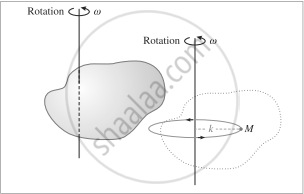
\includegraphics[scale=0.5]{gyration}

   The moment of inertia (MI) of body about a given roataion 
   axis depends upon(i) the mass of the body and (ii) the 
   distribution of mass about axis of roataion. These two factors
   can be seperated by expressing the MI as the product of the
   mass(M) and the square of a particular distance(k) from the 
   axis of roataion. This distance is called the radius of
   gyration and is defined as given above. Thus,
   \begin{equation}
   	I = \sum_{i} m_ir_i^2 = Mk^3 
   \end{equation}
   \begin{equation}
	   \therefore k = \sqrt{\frac{I}{M}}
   \end{equation}
   Physical significance: The radius of gyration is less if I is
   less, i.e., if the mass is distributed close to the axis;
   and it is more if I is more, i.e. if the mass is distributed
   away from the axis. Thus, it gives an idea about the 
   distribution of mass about the axis of roataion.

   \subsection{A uniform disc and a hallow right circular cone
   have the same formula for their moment of inerti when 
   rotating about their central axes. Why is it so?}
   A uniform disc and a hollow right circular cone have the 
   same formula for their moment of inertia.\\
   $MI = mr^2/2$ \\
   This is becaue when a hollow right circular cone is cut 
   along its slanting side and the metal is stretched out, you
   will find that the surface of the cone will form a circle.
   This shape is the same as the shape of disc, which is also
   circle. Hence they both have same forula for MI.

   \subsection{While driving along an unbanked circular road, a
   two wheeler rider has to learn with vertical. Why is it so?
   With what angle the rider has to lean? Derive the relevant
   expression. Why such a leaning is not neccessary for a four
   wheeler?}
   \begin{enumerate}
	\item When a bicyclist takes a turn along an unbanked
	road, the force of friction $\vec{f}_s$ prodvides the
	centripetal force; the normal reaction of the road
	$\vec{N}$ is vertically up. If the bicyclist does not
	learn inward, there will be an unbalanced outward
	torque about the centre of gravity, $f_s.h$, due to
	the frciton force that will topple the bicyclist 
	outward. The bicyclist must lean inward to counteract
	this torque (and not to generate a centripetal force)
	such that the opposite inward torque of the couple 
	formed by $\vec{N}$ and weight $\vec{g}$, $mg.a = 
	f_s.h_1$ \\ \\
	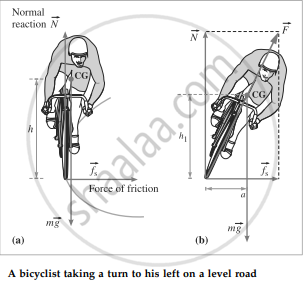
\includegraphics[scale=0.5]{bicyclist}

	\item Since the force of friction provides the
	centripetal force, 
	\begin{equation}
		f_s = \frac{mv_2}{r}
	\end{equation}
	If the cyclist leans from the vertical by an angle 
	$\theta$, the angle between $\vec{N}$ and $\vec{F}$
	\begin{equation}
		tan \theta = \frac{mv_2 / r}{mg} = 
		\frac{v^2}{gr}
	\end{equation}
	Hence, the cyclist must lean by an angle
	\begin{equation}
	    	\theta = \tan^-1 = (\frac{v^2}{gr})
	\end{equation}

	\item When a car takes a turn along a level road, apart
	from the risk of skidding off outward, it also has a
	tendency to roll outward due to an outward torque, it 
	also has a tendency to roll outward due to an outward
	torque about the centre of gravity due to the friction
	force. But a car is an extended object with four wheels.
	So, when the inner wheels just get lifted above the
	ground, it can be counterbalanced by a restoring
	torque of the couple formed by the normal reaction (on
	the outer wheels) and the weight. Consider a car of mass
	m taking turn of radius r along a level raod. As seen
	from an intertial frame of referance, the forces acting
	on the car are:
	\begin{enumerate}
		\item the lateral limiting force of static 
		friction $\vec{f}$ on the wheels - acting along
		the axis of the wheels and towards the center of
		the circular path which provides the neccessary 
		centripetal force.
		\item the weight $\vec{m}g$ acting vertically 
		downwards at the centre of gravity (C.G.)
		\item the normal reaction $\vec{N}$ of the road
		on the wheels, upwards effectively at the C.G.
		Since the maximum centripetal force = limiting
		force of static friction,
		\begin{equation}
			ma_r = \frac{mv^2}{r} = f_s
		\end{equation}
		In a simplified rigid-body vehicle, we consider
		only two parameters - the height h of the C.G.
		above the ground and tge average distance b
		between the left and right wheels called the 
		track width.\\\\

		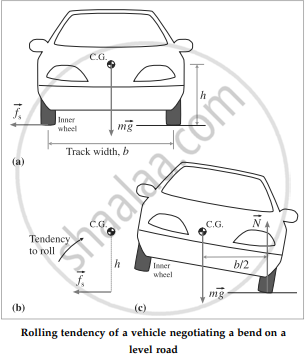
\includegraphics[scale=0.5]{rolling} \\\\

		The friction force $\vec{f}_s$ on the wheels
		produces a torque $\tau_t$ that tends to overturn
		/rollover the car abut the outer wheel in the
		above figure(b). Rotation about the fron to back
		axis is called roll.
		\begin{equation}
			\tau_t = f_s.h = (\frac{mv^2}{r}h)
		\end{equation}
		When the inner wheel just gets lifted above the
		ground, the normal reaction $\vec{N}$ of the road
		acts on the outer wheels but the weight continues
		to act at the C.G. Then, the couple formed by the
		normal reaction and the weight produces a 
		opposite torque $\tau_r$ which tenfs to restore 
		the car back on all four wheels in the above
		figure(b).
		\begin{equation}
			\tau_r = mg.\frac{b}{2}
		\end{equation}	
		The car does not topple as longas the restoring
		torque $\tau_r$ counterbalances, the toppling
		torque $\tau_r$ . \\
		Thus, to avoid the risk of rollover, the maximum
		speeed that the care can have is given by
		\begin{equation}
			(\frac{mv^2}{r})h = mg.\frac{b}{2} 
		\end{equation}
		\begin{equation}
			\therefore v_max = \sqrt{\frac{rbg}{2h}}
		\end{equation}
		Thus, the vehicle to roll when the radial 
		acceleration reaches a point where inner wheels
		of the four-wheeler are lifted off of the ground
		and the vehicle is rotated outward. A rollover
		occurs when the gravitational force $\vec{mg}$
		passes through the pivot point of the outer 
		wheels, i.e the C.G. is above the line of contact
		of the outer wheels. Equation(3) shows that this
		maximum speed is high for a car with larger track
		widtg and lowwer center of gravity.
	\end{enumerate}
   \end{enumerate}

   \subsection{Using energy conservation, derive the expression
   for the minimum speeds at different loctions along a vertical
   circular motion controlled by gravity.}
   Consider a particle of mass m attached to a string and
   revolved in a vertical circle of radius r. At every instant of
   its motion, the particle is acted upon by its weight 
   $\vec{mg}$ and the tesnion $\vec{T}$ in the string. Let $v_2$
   be the speed of the body and $T_2$ be the tesnion in the 
   string at the lowest point B. We take the referance level 
   for the zero potential energy to be bottom of the circle.
   Then, the body has only kinetic energy $\frac{1}{2}mv_2^2$
   at the lowest point.
   \begin{equation}
   	T_2 = \frac{mv_2^2}{r} + mg
   \end{equation}
   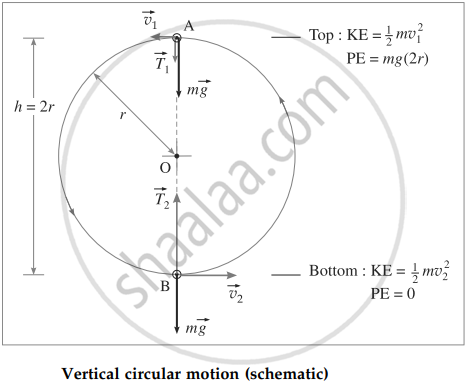
\includegraphics[scale=0.5]{vcm} \\
   and the total energy at the bottom - KE + PE
   \begin{equation}
	   \frac{1}{2}mv_2^2 + 0
   \end{equation}
   Let $v_1$ be the speed and $T_1$ the tension in the string
   at the highest point A. As the body goes from B to A, it 
   rises through a height h = 2r.
   \begin{equation}
	   \therefore T_1 = \frac{mv_1^2}{r} - mg
   \end{equation}
   and the total energy at A = KE + PE
   \begin{equation}
	   = \frac{1}{2} mv_1^2 + mg(2r)
   \end{equation}
   Then, from Eqs(15) and (17),
   \begin{equation}
	   T_2 - T_1 = \frac{mv_2^2}{r} + mg - (\frac{mv_1^2}
	   {r} - mg)
   \end{equation}
   \begin{equation}
	   = \frac{m}{r} (v_2^2 - v_1^2) + 2mg
   \end{equation}
   Assuming that the total energy of the body is conserved,
   the total energy at the bottom = total energy at the top \\
   Then, from Eqs(16) and (18)
   \begin{equation}
	   \frac{1}{2}mv_2^2 = \frac{1}{2}mv_1^2 + mg(2r)
   \end{equation}
   \begin{equation}
   	\therefore v_2^2 - v_1^2 = 4gr
   \end{equation}
   Subsittuting this in eq(20),
   \begin{equation}
	   T_2 - T_1 = \frac{m}{r}(4gr) + 2mg
   \end{equation}
   \begin{equation}
   	= 4mg + 2mg = 6mg
   \end{equation}
   Therefore, the difference in the tensions in the string at
   the highest and lowest points is 6 times the weight of the
   body.
\end{document}
